\section{Tensorflow遇上Kubernetes}
\label{sec:tensorflow-on-kubernetes}

\begin{frame}
  \begin{center}
    \Huge{\textcolor{red}{Tensorflow遇上Kubernetes}}
  \end{center}
\end{frame}

\subsection{Tensorflow On Kubernetes}

\begin{frame}{容器化高性能计算集群}
  \begin{figure}
    \centering
    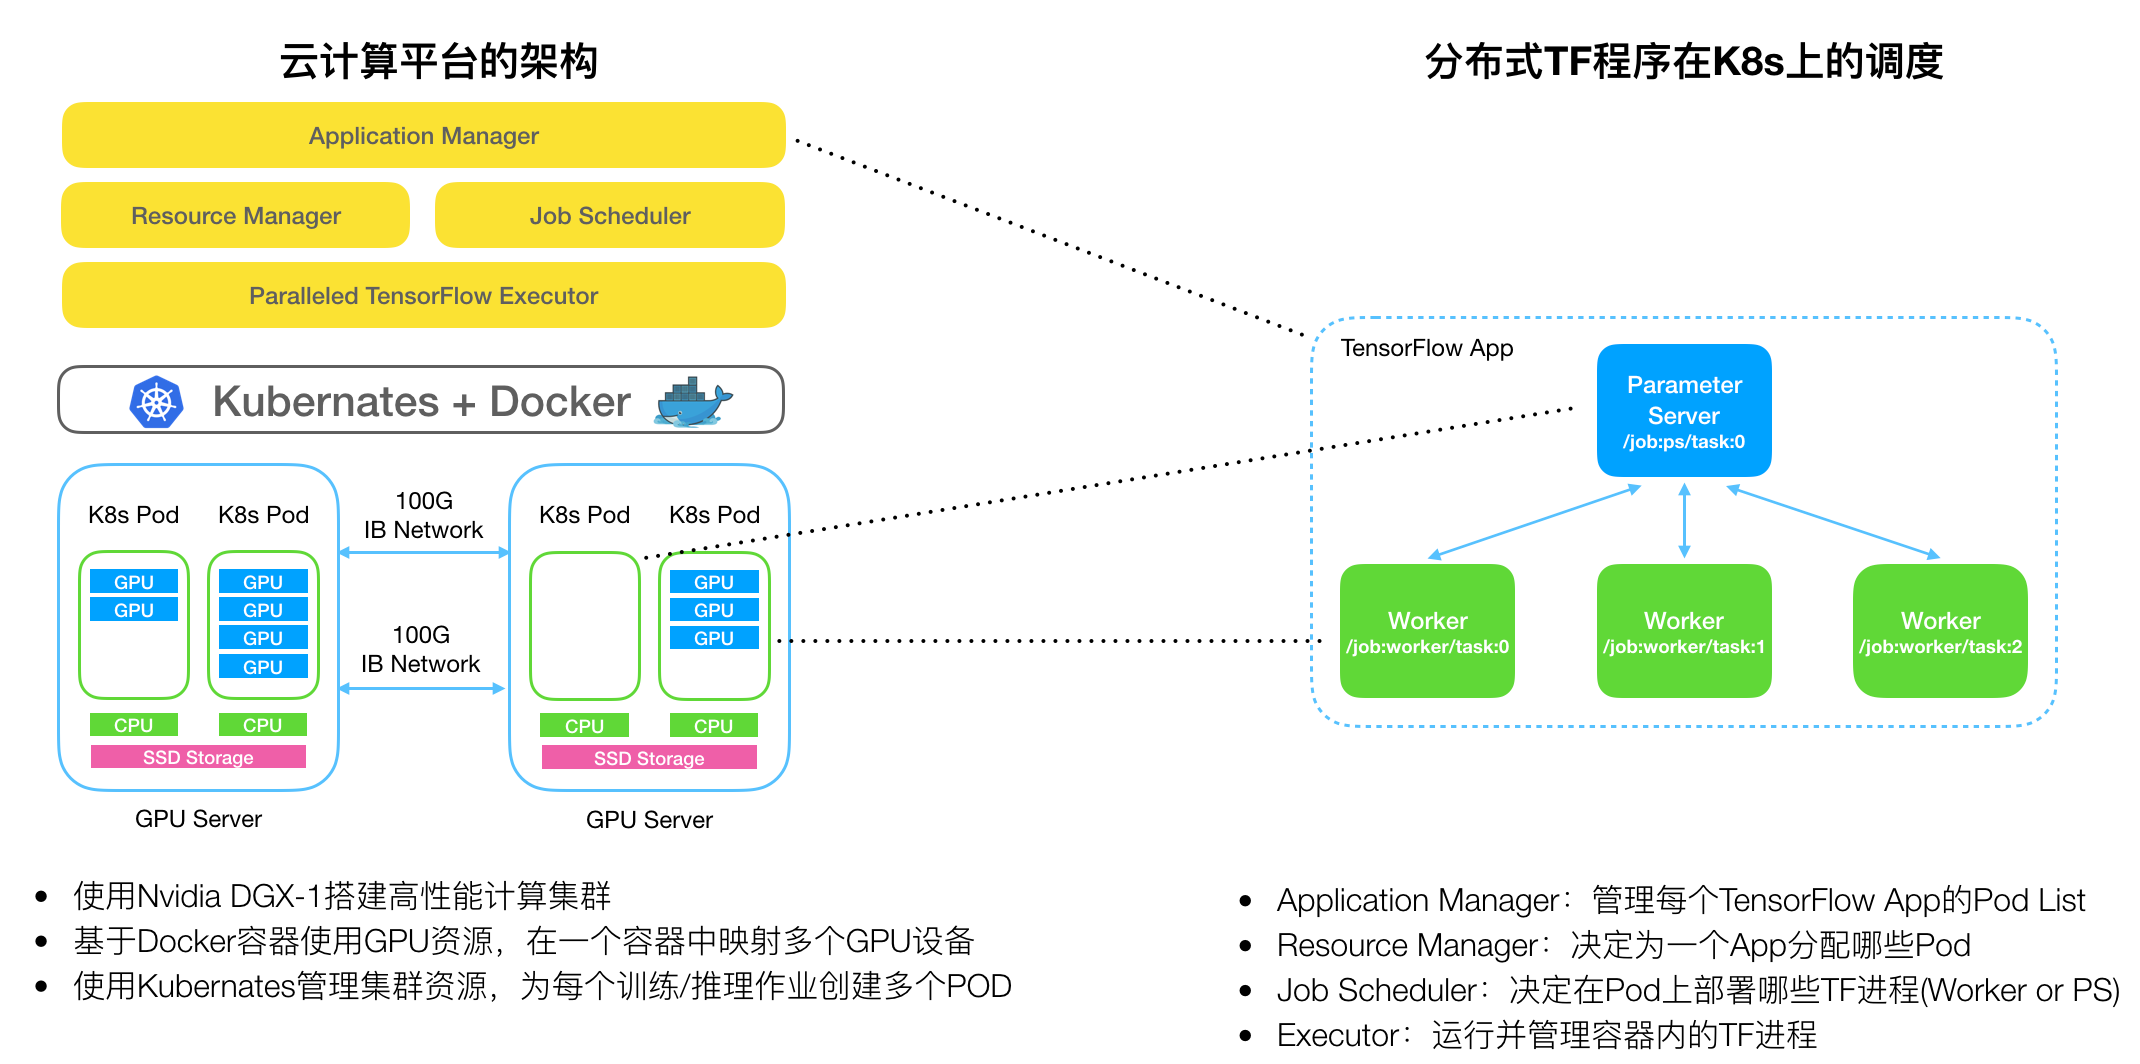
\includegraphics[width=1.0\textwidth]{tf-on-k8s.png}
  \end{figure}
\end{frame}

\begin{frame}{扩展K8s支持GPU和RMDA网络}
  \begin{figure}
    \centering
    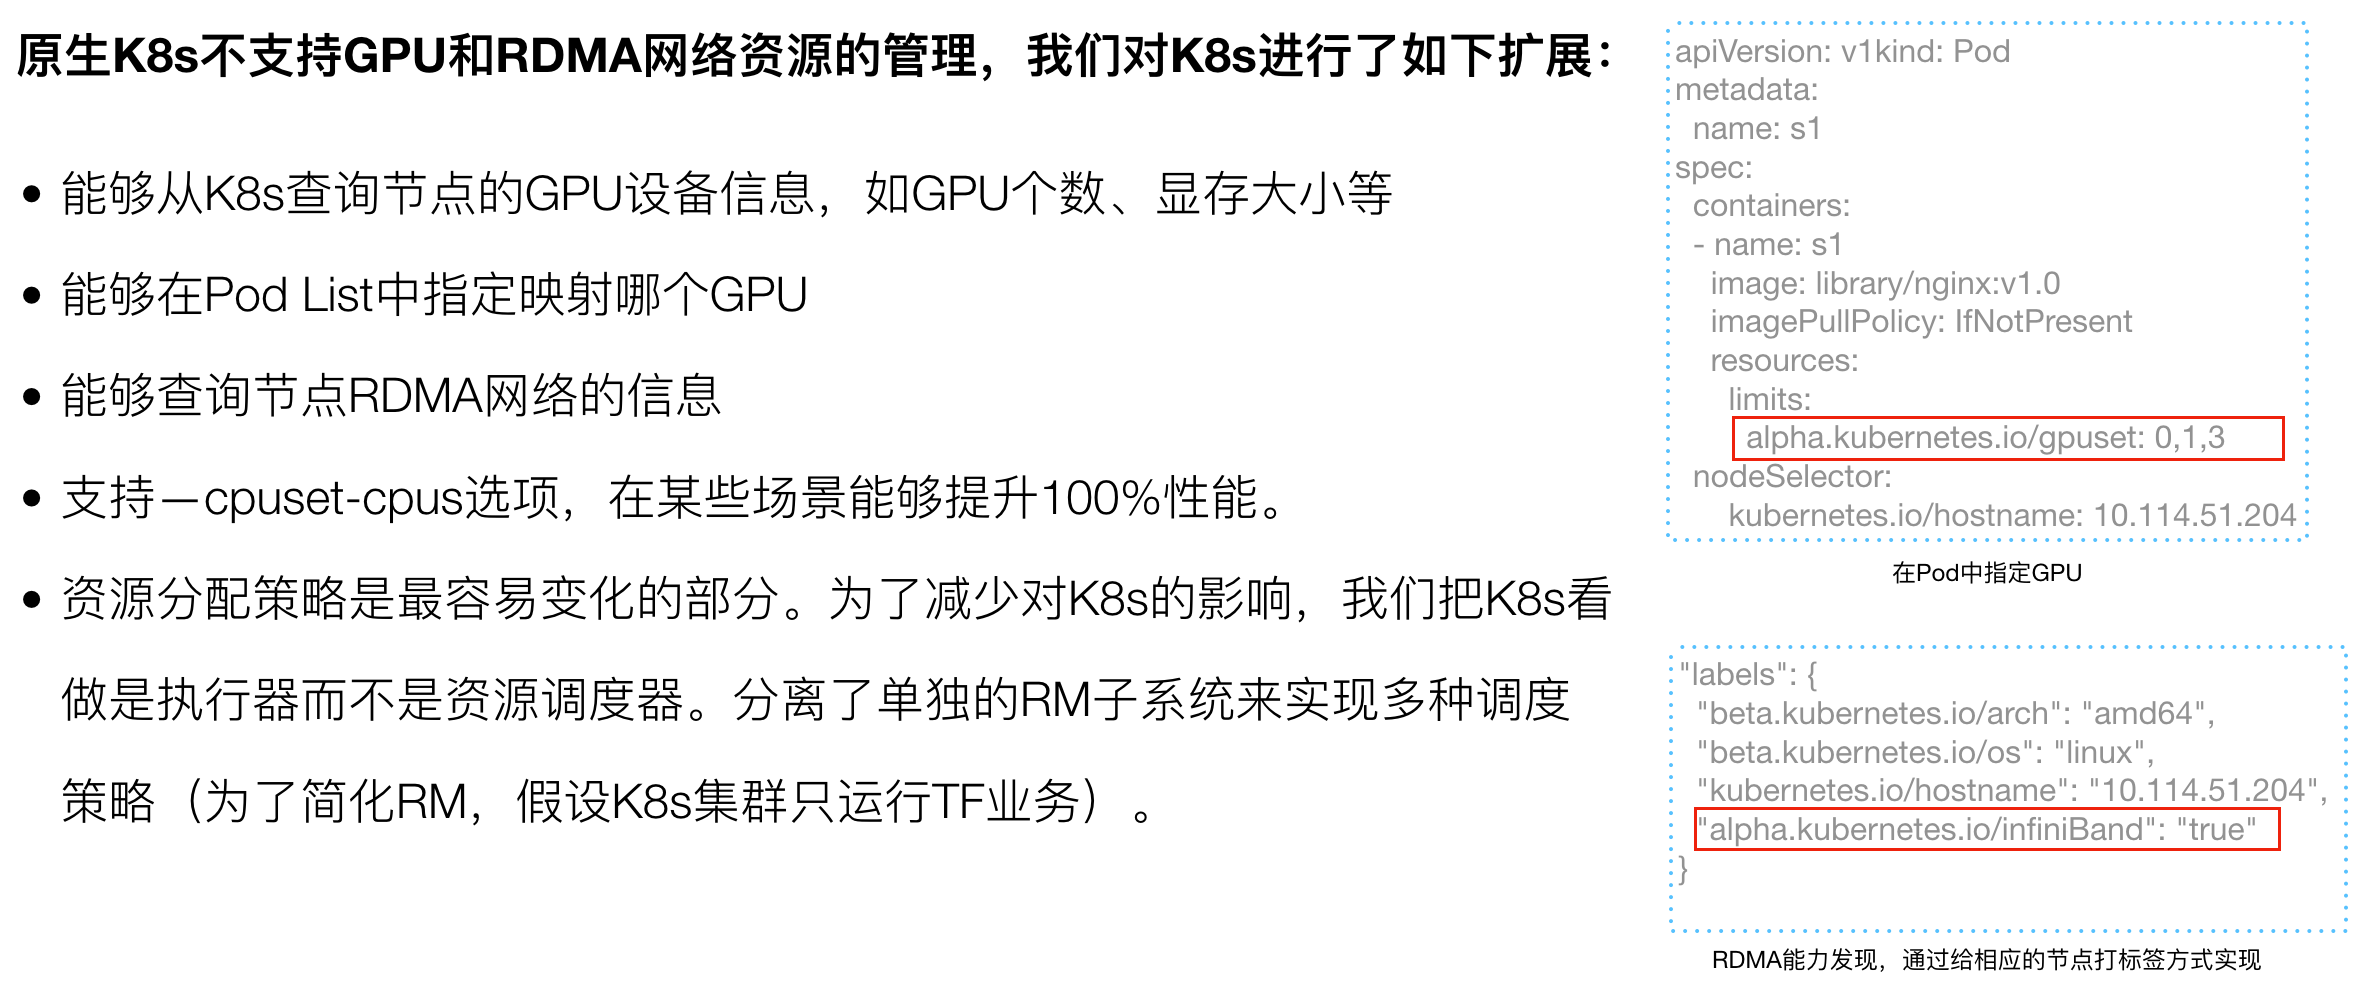
\includegraphics[width=1.0\textwidth]{k8s-gpu-extension.png}
  \end{figure}
\end{frame}

\begin{frame}{在云上执行分布式TF计算}
  \begin{figure}
    \centering
    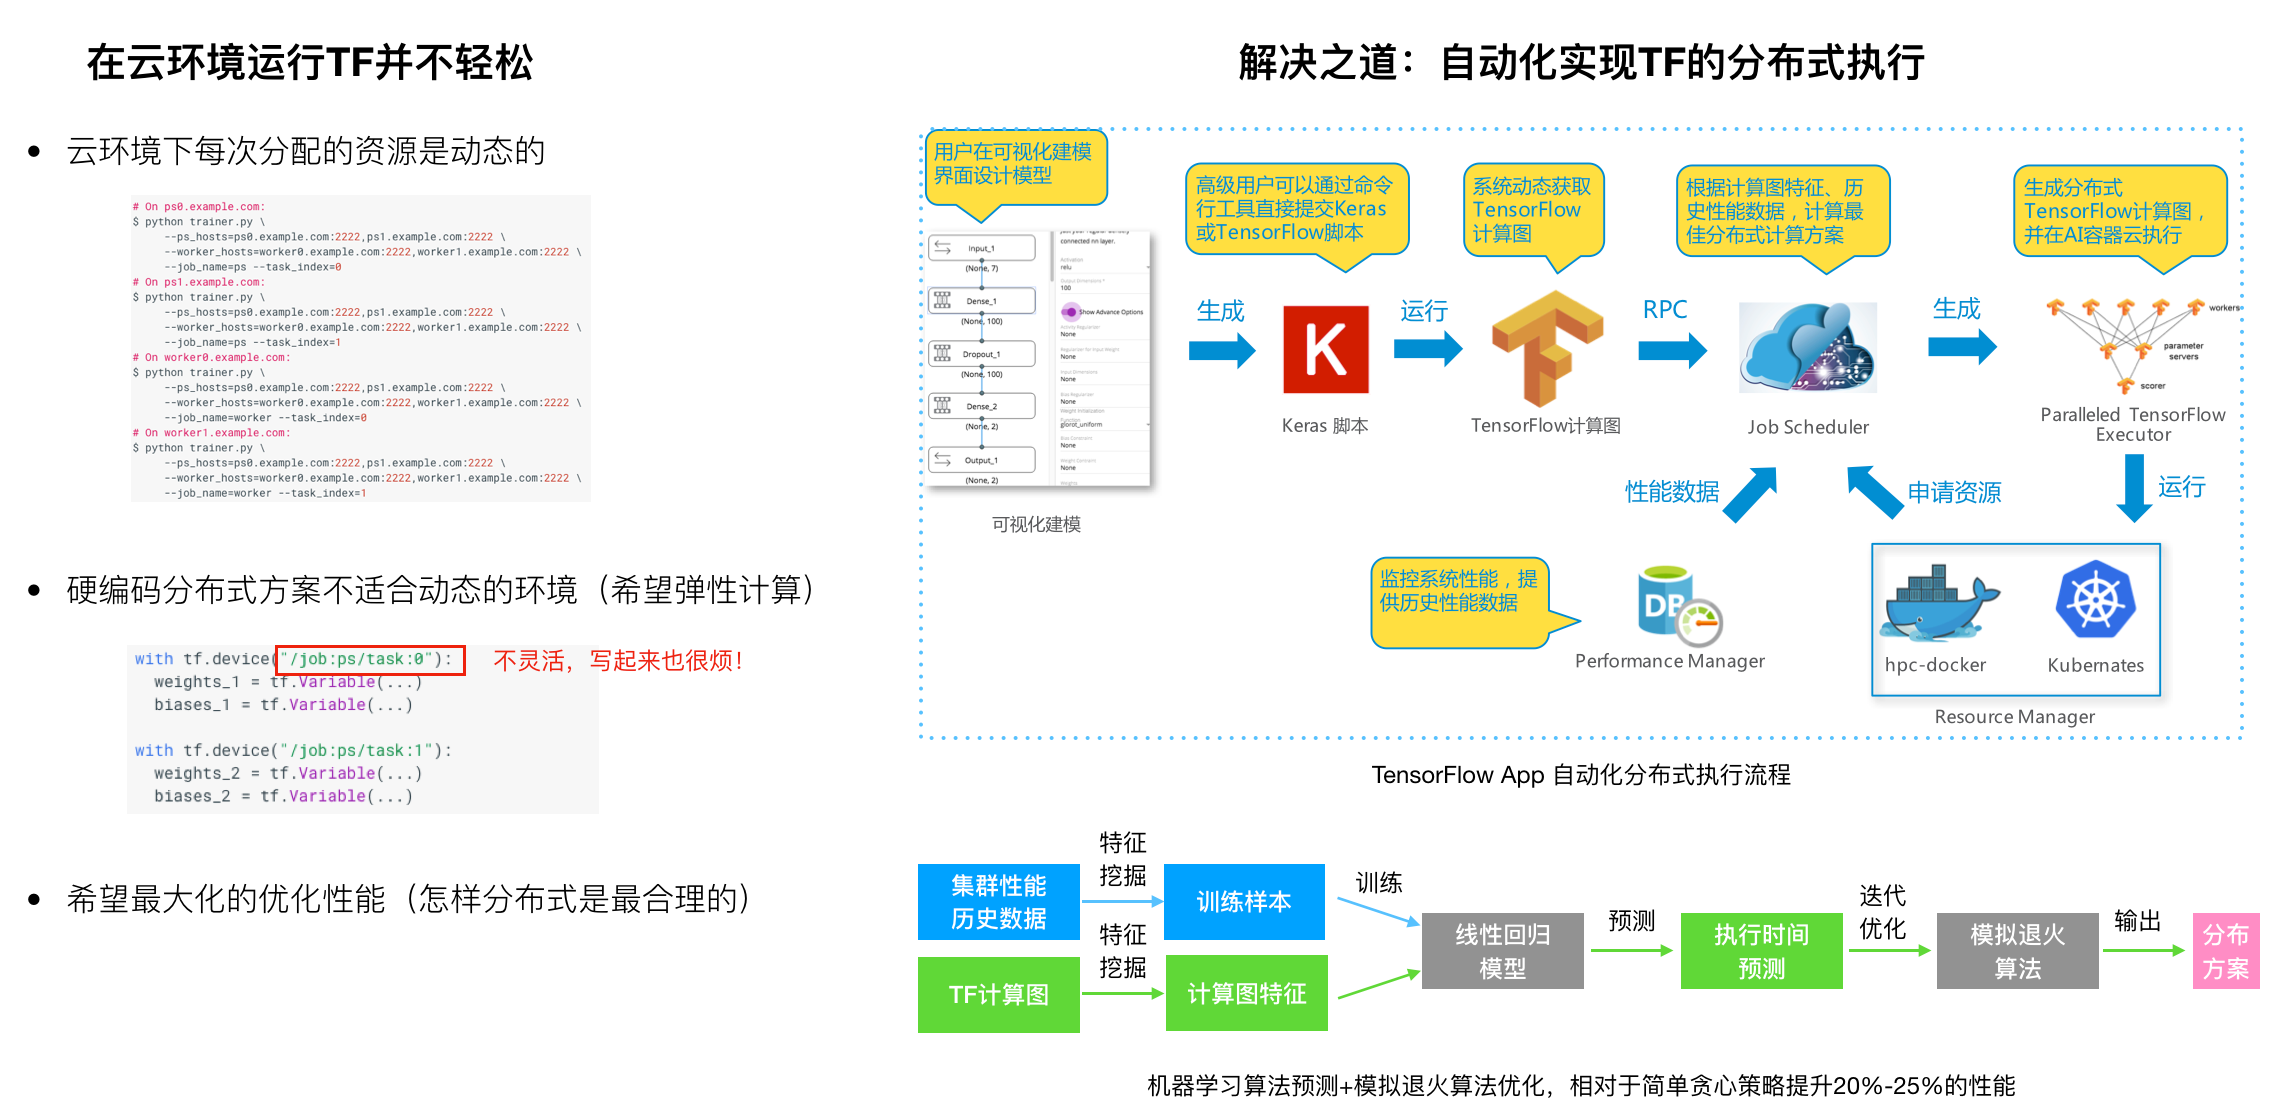
\includegraphics[width=1.0\textwidth]{auto-placement-workflow.png}
  \end{figure}
\end{frame}

\begin{frame}{计算模型优化}
  \begin{figure}
    \centering
    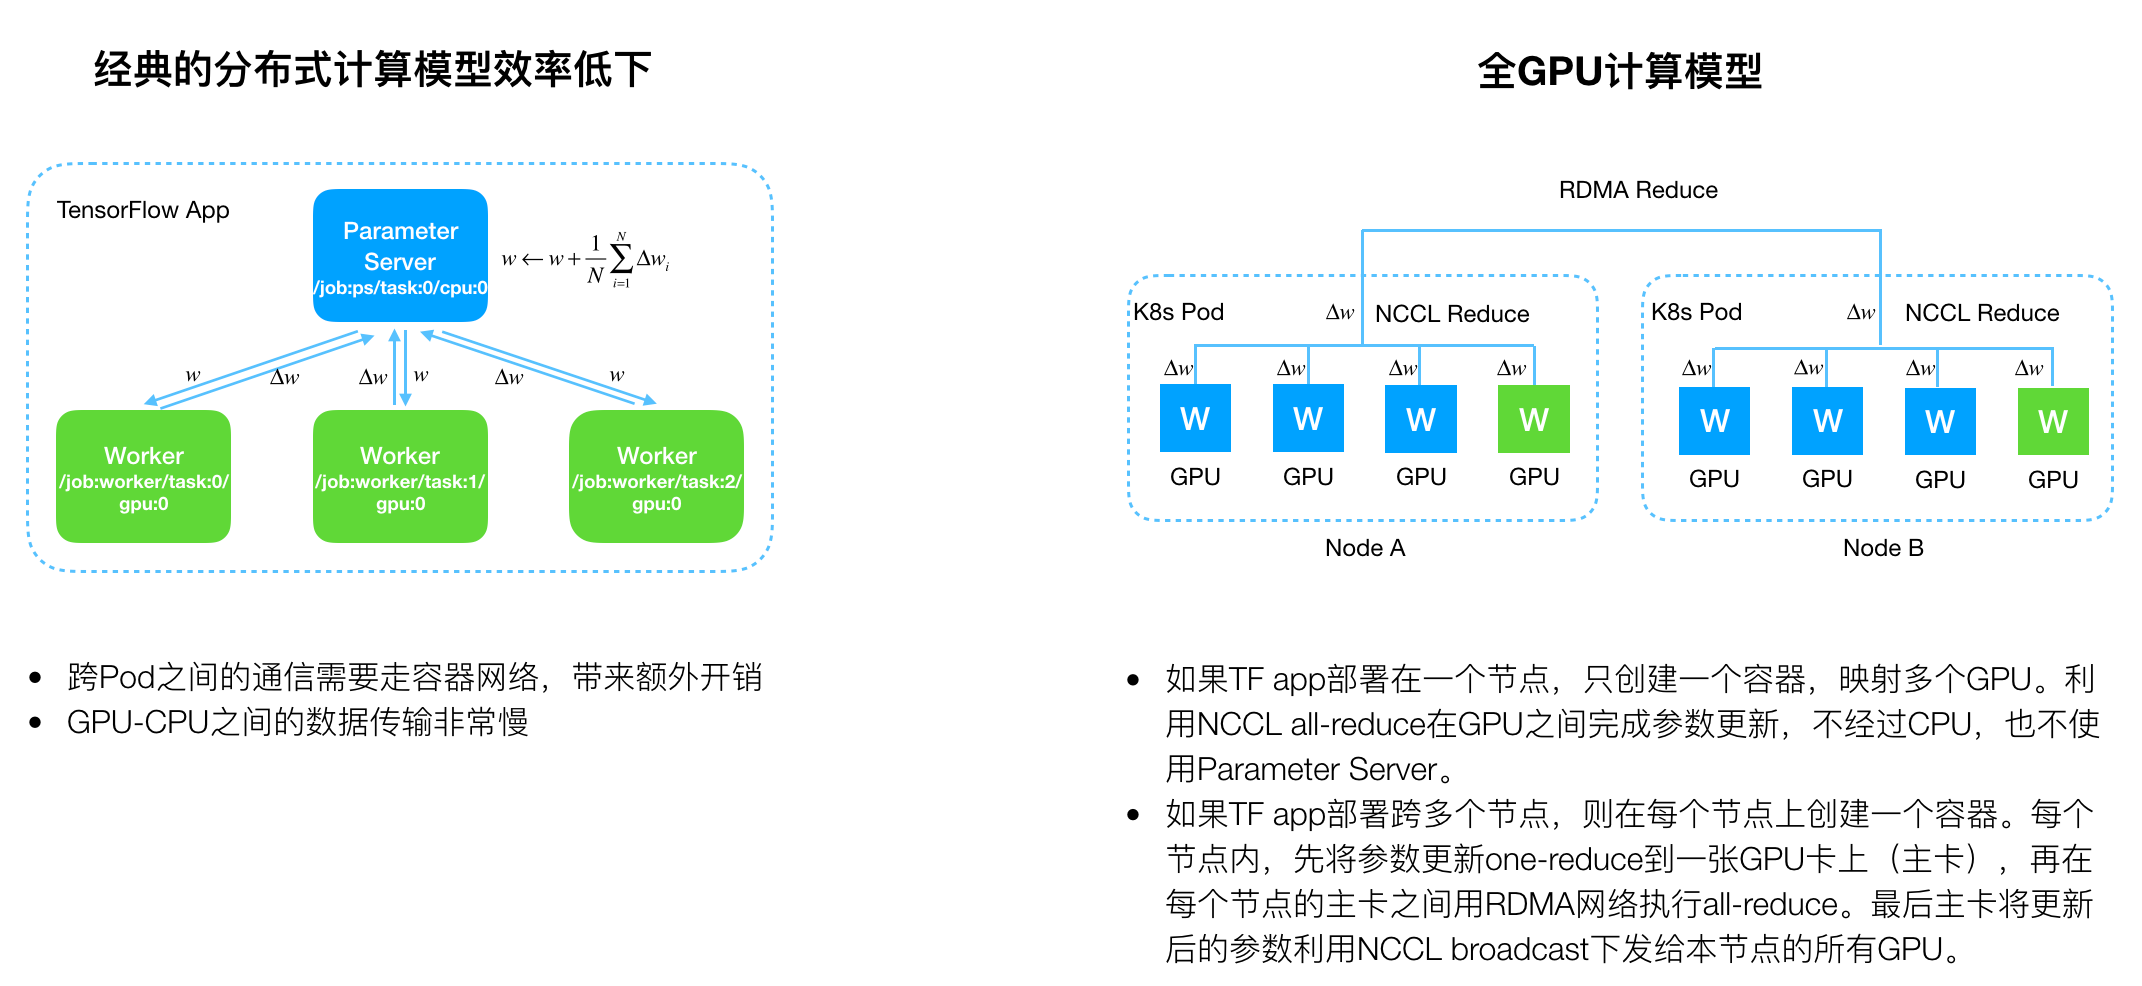
\includegraphics[width=1.0\textwidth]{optimize-performance.png}
  \end{figure}
\end{frame}
